\chapter{Wstęp}
\section{Wprowadzenie}

Algorytmy automatycznej kontroli głośności(AGC) są ważnym elementem współczesnych systemów przetwarzania sygnałów audio. Celem stosowania takiego algorytmu jest utrzymanie stałej głośności wszystkich mówców w danym systemie. Konkretnym przykładem zastosowania są wideokonferencje \cite{agc_application}, które z uwagi na sytację pandemiczną na świecie zyskały ogromną popularność. Z uwagi na różne czułości mikrofonów uczestników, różną głośność mówienia i odległość od mikrofonu, uczestnicy mogą odczuwać nieprzyjemne dla ucha fluktuacje głośności. Algorytm AGC redukuje te efekty. Ważne jest aby takie algorytmy skutkowały wysokim poziomem sygnału do szumu(SNR) jak i wysokim stosunkiem sygnału do szumu do pozostałych interferencji.

Najprostszym rozwiązaniem jest zastosowanie systemu jednokanałowego \cite{Archibald2008}. W takim systemie możlie jest tylko sterowanie głośnością sygnału wejściowego, na podstawie chwilowej wartości obwiedni. Uniemożliwia on jednak różny poziom wzmocnienia dla różnych mówców i usunięcie interferencji, jeśli współistnieją one w czasie z głównym sygnałem.

Rozwiązaniem bardziej skomplikowanym, zarówno od strony sprzętowej, programistycznej i czasu obliczeń jest użycie systemu z wieloma mikrofonami. Taki system umożliwia pożądane rozróżnienie między mówcami i eliminację interferencji \cite{Thiergart2013}. W systemie takim możliwa jest estymacja kierunków nadchodzenia fali, a co za tym idzie mocy nadchodzącej z wybranych stron i zastosowanie odpowiednich filtrów, które wzmacniają sygnał z żądanych kierunków.

W tej pracy skupiono się właśnie na drugim z wymienionych rodzajów algorytmów AGC. W pracy zostanie przedstawiona praktyczna implementacja bazująca na nagraniach z macierzy mikrofonowych.

\begin{figure}[h]
    \centering
    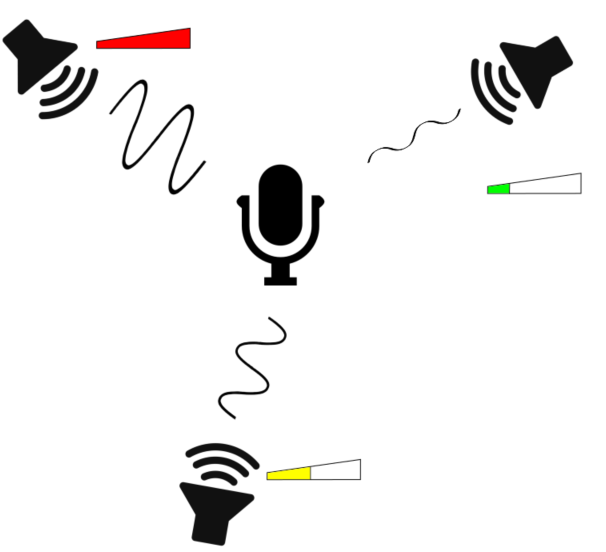
\includegraphics[width=\textwidth]{Images/setup.png}
    \caption{Graficzna reprezentacja problemu}
    \label{fig:setup}
\end{figure}

\section{Cel}
Celem pracy inżynierskiej była praktyczna implementacja istniejącego algorytmu AGC z tłumieniem tła akustycznego, wraz z estymacją kierunku nadchodzenia fali. Wybrany algorytm powinien spełniać cechy wymienione w poprzedniej sekcji,tj. pozwala na regulację głośności nagrania zarówno w czasie jak i między mówcami i minimalizację zakłóceń. Z tego powodu zdecydowano się na użycie tak zwanego filtra LCMV. Opracowany algorytm w założeniu nie ma być algorytmem czasu rzeczywistego. Powinien wykonywać żądane operacje bazując na nagraniach z macierzy mikrofonowej.

\section{Zakres wykonanej pracy}
Pierwszym z etapów pracy inżynierskiej było zapoznanie się autora pracy z dostępnymi publikacjami opisującymi zarówno tematykę AGC \cite{Thiergart2013}, \cite{Archibald2008} jak i generalną tematykę przetwarzania sygnałów dla macierzy czujników \cite{Benesty2008} i wybór metody. 
Następnie dokonany wyboru środowiska pracy- języka Python wraz z paczką NumPy \cite{numpy}. Szczegółowy opis użytych narzędzie znajduje się w \ref{chapter-4}. Następnie autor pracy napisał symulator umożliwiający generację sygnałów mikrofonowych. Dalsza część realizacji pracy obejmowała- zaplanowanie praktycznej implementacji systemu, wykonanie tej implementacji i testy przy użyciu symulatora. 

